%% $RCSfile: proj_report_outline.tex,v $
%% $Revision: 1.2 $
%% $Date: 2010/04/23 02:40:16 $
%% $Author: kevin $

\documentclass[11pt, a4paper, twoside, openright]{report}


\usepackage{float} % lets you have non-floating floats

\usepackage{hyperref} % for typesetting urls

%
%  We don't want figures to float so we define
%
\newfloat{fig}{thp}{lof}[chapter]
\floatname{fig}{Figure}

%% These are standard LaTeX definitions for the document
%%                            
\title{Security Visualisation Tools}
\author{Leliel Trethowen}

%% This file can be used for creating a wide range of reports
%%  across various Schools
%%
%% Set up some things, mostly for the front page, for your specific document
%
% Current options are:
% [ecs|msor]              Which school you are in.
%
% [bschonscomp|mcompsci]  Which degree you are doing
%                          You can also specify any other degree by name
%                          (see below)
% [font|image]            Use a font or an image for the VUW logo
%                          The font option will only work on ECS systems
%
\usepackage[image,ecs]{vuwproject}

% You should specifiy your supervisor here with
%     \supervisor{Firstname Lastname}
\supervisors{Ian Welch, Stuart Marshall}

% Unless you've used the bschonscomp or mcompsci
%  options above use
\otherdegree{Bachelor of Engineering(Hons)}
% here to specify degree

% Comment this out if you want the date printed.
\date{}

\begin{document}

% Make the page numbering roman, until after the contents, etc.
\frontmatter

%%%%%%%%%%%%%%%%%%%%%%%%%%%%%%%%%%%%%%%%%%%%%%%%%%%%%%%

%%%%%%%%%%%%%%%%%%%%%%%%%%%%%%%%%%%%%%%%%%%%%%%%%%%%%%%

\begin{abstract}

Detecting malicious attempts to access computers is difficult with current tools. Many current tools do not give the user the right information to find and analyse possible attempts. Visual analytics approaches support users to find the information they need. An effective visual analytics tool would improve detection rates.

\end{abstract}

%%%%%%%%%%%%%%%%%%%%%%%%%%%%%%%%%%%%%%%%%%%%%%%%%%%%%%%

\maketitle

%\chapter*{Acknowledgments}\label{C:ack} 
Any acknowledgments should go 
in here, between the title page and the table of contents.  The 
acknowledgments do not form a proper chapter, and so don't get a 
number or appear in the table of contents.

\tableofcontents

% we want a list of the figures we defined
\listof{fig}{Figures}

%%%%%%%%%%%%%%%%%%%%%%%%%%%%%%%%%%%%%%%%%%%%%%%%%%%%%%%

\mainmatter

%%%%%%%%%%%%%%%%%%%%%%%%%%%%%%%%%%%%%%%%%%%%%%%%%%%%%%%

% individual chapters included here
\chapter{Introduction}\label{C:intro}

Maintaining access control and information security has been an ongoing problem since people first realised that information is valuable and can be controlled. This problem quickly became apparent in networked systems after their invention and adoption outside the lab.

As networks have become ubiquitous and essential for modern life, threats to the integrity of networks and data have multiplied and diversified extensively. 
This proliferation of threats has lead to the design and use of tools intended to secure systems, and monitor for intrusions \cite{zhang2012survey}. Intrusions are defined loosely here as access to systems resources for purposes contrary to the intended use of the system, or access to the system by an unauthorised person (often an unauthorised person is also misusing the system). This may be as innocuous as browsing facebook while at work, or much more severe. Ie: stealing secrets or using the systems to run a botnet. Security policies exist as a formal statement of the intended uses of the system, and examples of uses considered malicious. The formal statement of acceptable and unacceptable system uses is extremely useful as it allows for configuring systems to deny many forms of intrusion. ie: denying remote login with an administrator account. 

There are two main forms of malicious user that should be considered. The outsider, these people do not have any legitimate access to the system. Obviously, their attempts should be denied. The second form is the insider attack. These may be significantly harder to detect as the attacker has legitimate access rights to the system, but is using them for purposes not authorised by the system owners.

Insider attacks are by far more difficult to combat effectively by technical means, as the user in question requires access to some or all of the systems to perform their jobs. This prevents simple solutions such as blanket denial of access. Further, this complicates detection of unauthorised access by obscuring illegitimate uses of the system within legitimate uses which should not be interfered with.

There are two main methods of operation for Intrusion Detection Systems(IDS).
Rule based systems, which flag any attempt that matches defined rules as malicious. These systems are extremely effective at detecting and blocking known attack patterns, particularly for outsider access as rules are relatively simple to write once the signature patterns in the attack are known. Insider attacks are more difficult to control with rules based systems, as blanket access blocks are often not suitable. 

Anomaly based detection systems use techniques from machine learning to automatically classify incoming events as normal or anomalous. Normal events are ignored, while anomalous events are flagged for operator attention. These systems have some obvious advantanges. Firstly they're able to recognise new intrusion methods, as they will appear as an anomaly, However, they're not able to provide much if any context for these events. Rule based systems at least identify which rule was matched. Anomaly detection systems are harder to disguise existing intrusions from, as their classification systems are flexible enough to recognise small changes in patterns. Rule based systems cannot do this as easily.

Both approaches are used heavily in monitoring network traffic generally. While somewhat successful, both approaches potentially suffer from false positives (Anomaly based more frequently than rules based) and possibly more worrying, false negatives. 

False negatives are quite obviously undesireable as each represents an intrusion that went undetected and potentially un-countered. Note that not all undetected intrusions will achieve their goals, however security administrators are not able to effectively ensure the vulnerabilities used are addressed, as they may remain unaware of the intrusion indefinitely, unless traces are left elsewhere in the system.

Large numbers of false positives are a serious problem for security systems as the quickly undermine user's trust in the systems \cite{stanton1994human}. Many IDS offer very limited forms of alerting with email most used, and SMS messaging an option for critical alerts. The limited range of sensory urgency available to IDS alerting mechanisms is problematic, as it causes a mismatch between the apparent and actual import of a message \cite{stanton1994human}. 

These factors leave a significant problem for security professionals. How do we ensure that actual intrusions are being detected, despite ever advancing intrusion techniques and rapidly growing size and complexity of networks to defend?. As I will show in Chapter \ref{C:back}, existing approaches fail to meet the goals laid out for this project. Many either do not scale well to large networks or easily cause information overload. Information overload creates an effect where the monitoring system looks a bit like a christmas tree. lots of pretty blinking lights, but no meaning. Many others fail to reveal important context about the events they flag. 

This project takes a data visualisation approach to solving the issue of detecting intrusion attempts, attempting to use human ability to spot and interpret novel patterns in data, without stripping context from the existing attempts. 

Due to time limitations, I will be restricting the focus of this tool from general network traffic, to remote access attempts through the SSH protocol. SSH is a commonly used protocol for server control and administration, as well as remote access and file sharing. ports used for SSH traffic are often the focus of intrusion attempts.

The overall goal is to create a tool that allows security adminstrators to effectively monitor remote access attempts to their systems for intrusions. 
In order to support this aim, several subidiary goals must be achieved.

\begin{enumerate}
\item{Clearly show patterns in login data.}
\item{Avoid information overload (the "christmas tree" effect).}
\item{Provide context for events.}
\item{Scale to many machines and millions of events.}
\end{enumerate}

Chapter \ref{C:back} discusses related works and reqirements for the project. Progress to date is discussed in chapter \ref{C:progress}, this is broken down into two major areas, design and evaluation. In chapter \ref{C:future} I discuss plans for the remaining work in three sections, Design, Implementation, and a timeline.

\chapter{Related Work}\label{C:back}

Much related work has been done in two major areas. Data mining focused techniques with visualisations used to explore the results of data mining, and visualisation driven techniques. Most visualisation driven techniques still contain significant datamining tools. Relatively little work has been done directly on access or system log visualisation, with research preferring to focus on network intrusion detetection logs. For the purposes of this section Intrusion Detection Systems(IDS) are treated as datamining systems. For anomaly based IDS this is straightforward, as they use traditional machine learning and datamining techniques to create classification systems for events. In rule based IDS, this is not so clear, as they apply pre-created rules. However, these rules are often created using data-mining techniques and serve to offer the same black box classification system as other data-mining software. I will be considering how each system discussed below meets the goals set out in Chapter \ref{C:intro}.

\subsection{Data Mining with Visualisation}

LogView \cite{4641277} is a visualisation tool designed to support undertstanding of information extracted through data-mining techniques applied to systems logs. The visualisation component uses treemaps to show clusters of events in a space efficient manner, with leaf nodes representing events, and branches showing clusters the events belong to. All leaf nodes are coloured in green, with shade darkening in 4 steps, representing  statuses OK, WARN, FAIL, OUTLIER in order.  The tool produced allows filtering based on time, and search terms. Time filtering shows only events occuring on the specified day in the map. Nodes matching search terms are highlighted red. Detailed information about a given event is available via mouseover. The simple filtering and interaction methods, coupled with very similar shades for clusters leaves the system very vulnerable to producing information overload in users. The overload potential grows rapidly as the logs grow, as there is very little information hiding present in this tool. 

\begin{figure}[tbh]
\fbox{\parbox[b]{.99\linewidth}{
\vskip 0.5cm
\centering 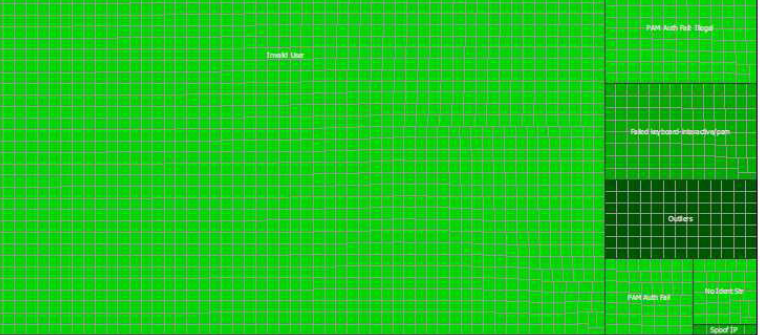
\includegraphics[scale=0.5]{tree.png}
\vskip 0.5cm}}
\caption{\protect\label{tree} LogView treemap of SSHD logs \cite{4641277}. Shades of green indicate severity of event.}
\end{figure}

A heirarchical system for visualising IDS logs \cite{itoh2006hierarchical} shows an interesting approach to the issue of context for IDS reports. Intrusion detection system messages are lacking in the context needed to support an evaluation of the priority and accuracy of the report. This tool shows the entire network under surveillance using a rectangle packing algorithm to group machines by subnets, the number of incidents sent and recieved from a given machine are displayed as a coloured bar rising out of the plane. This quickly leads to navigability and readability problems as the number of incidents reported grows. Simple filtering tools are available to limit by severity, time, IP and signature ID.
This system is highly reliant on an IDS system with both a low false positive, and false negative rate, as almost all information about the actual events is hidden, and no easy method to drill down to detailed information is provided.

A system log data mining approach is presented by W. Xu et al. \cite{Xu:2009:DLS:1629575.1629587}. This approach uses data mining and machine learning techniques heavily. Log syntax is automatically recovered through source code analysis, allowing the system to be applied to any source available software. Once log synatx is extracted, logs are parsed and machine learning algorithms used to perform feature extraction. Once the features were extracted the principle component analysis anomaly detection algorithm were applied to this data, to find interesting patterns in log messages. This approach identified many issues in the tested software, but was forced to be extended from a pure data-mining approach as users found the black box nature of data-mining algorithms caused difficulty in understanding why the results were as they are. To assist with this, a very simple decision tree visualisation was added, shown in Figure \ref{decision}. This visualisation was created with the intention of showing the logic used by the data-mining systems to give context for decisions. As the processing required for feature extraction and anomaly detection is highly parallel this approach readily scales to millions of entries, and shows very strong performance in detecting anomalous patterns in logs. However, from a security standpoint decision trees alone do not give sufficient context to easily determine if an anomaly represents an intrusion. This depends on much data not included in the raw logs.

\begin{figure}[tbh]
\fbox{\parbox[b]{.99\linewidth}{
\vskip 0.5cm
\centering 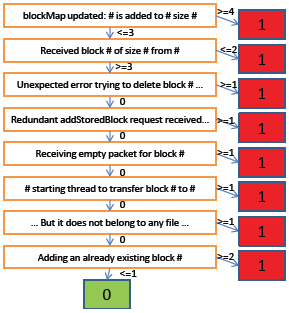
\includegraphics[scale=.75]{decisions.png}
\vskip 0.5cm}}
\caption{\protect\label{decision} Decision tree diagram \cite{Xu:2009:DLS:1629575.1629587}. Red 1's indicate anomalies, Green 0 indicates normal. labels on the edges show count thresholds for decisions.}
\end{figure}

\subsection{Visualisation Focused}

Picvis \cite{tricaud2008picviz} is a tool created to generate parallel co-ordinate plots of log data. Picviz offers tools to automate data extraction from several common log formats for use with their plot description language (pcl). This language allows a great deal of control over what variables are shown on a plot. Parallel co-ordinate plots can show strong clustering extremely well. However there are issues of scalability, as clusters and patterns can easily be hidden in background noise unless axes are well chosen. See Figure \ref{parallel}. Filtering tools are available to help address this limitation, but still require significant knowlege of the data structure and content. This tool would be excellent for confirmatory analyses however. 

\begin{figure}[tbh]
\fbox{\parbox[b]{.99\linewidth}{
\vskip 0.5cm
\centering 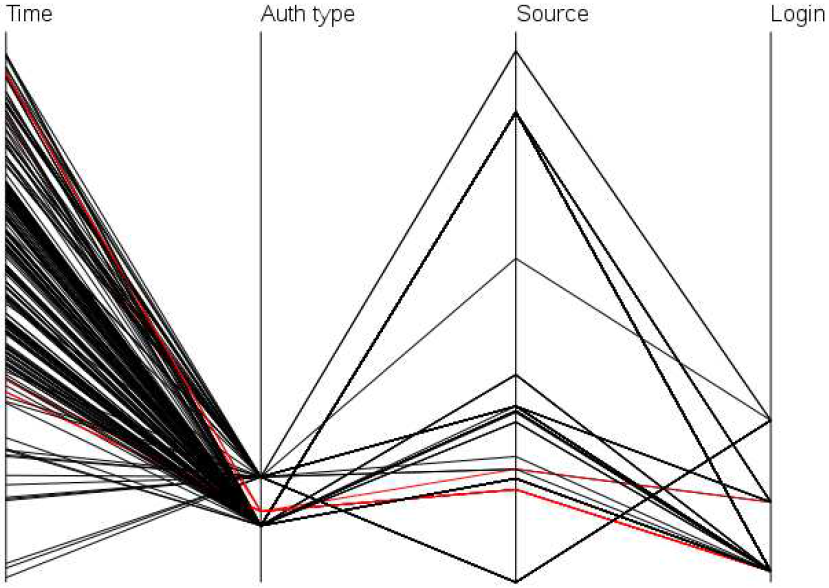
\includegraphics[scale=0.5]{parallel.png}
\vskip 0.5cm}}
\caption{\protect\label{parallel} Picviz parallel plots visualisation \cite{tricaud2008picviz} showing SSH logs.}
\end{figure}

Spiralview \cite{bertini2007spiralview} is a layout technique for timeseries data. Data is laid out in a spiral as shown in Figure \ref{spiral}. This technique has been used both for dynamic data streams \cite{chin2009visual} and analysis of static logs \cite{bertini2007spiralview}. In both applications strong promise is shown intially, as the spiral layout is intuitively expected to effectively reveal repeating patterns in time series data, such as intrusion detection system reports and access logs. However, the paper presenting the spiral technique for use in analysis of static logs does not attempt to evaluate the effectiveness with rigour \cite{bertini2007spiralview}. A rigorous evaluation of the spiral technique was performed in the paper proposing its use for dynamic datastreams \cite{chin2009visual}, However there are severe flaws in the presentation of this evaluation, as the table of results directly contradicts the text. 

\begin{figure}[tbh]
\fbox{\parbox[b]{.99\linewidth}{
\vskip 0.5cm
\centering 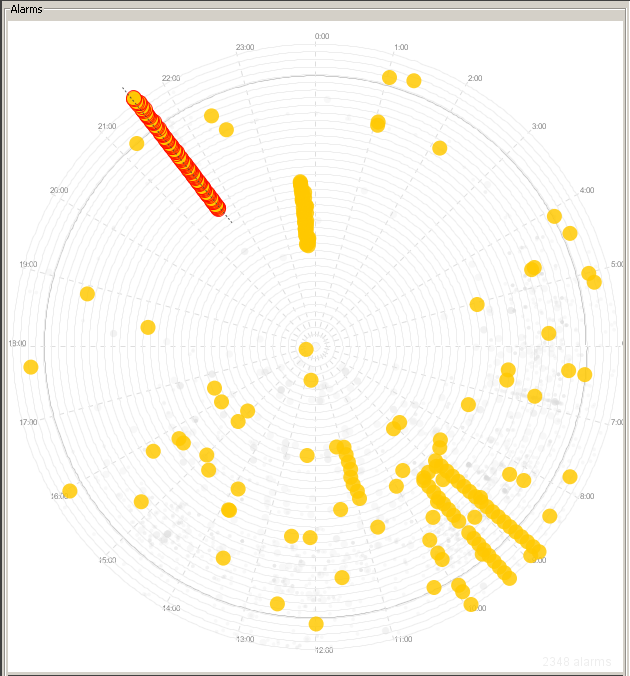
\includegraphics[scale=0.5]{spiral.png}
\vskip 0.5cm}}
\caption{\protect\label{spiral}Spiralview showing IDS logs over time. \cite{bertini2007spiralview}}
\end{figure}

Integrated visualisation system \cite{mukosaka2007integrated} is an IDS log based visualisation tool, focusing on attacks originating inside the monitored network, as these events are less well studied and have important security implications for the network. The tool provides a unified logical, geographic and temporal display of data, using three orthogonal planes. Multiple layouts of the three planes are available, with animated transitions. 

\begin{figure}[tbh]
\fbox{\parbox[b]{.99\linewidth}{
\vskip 0.5cm
\centering 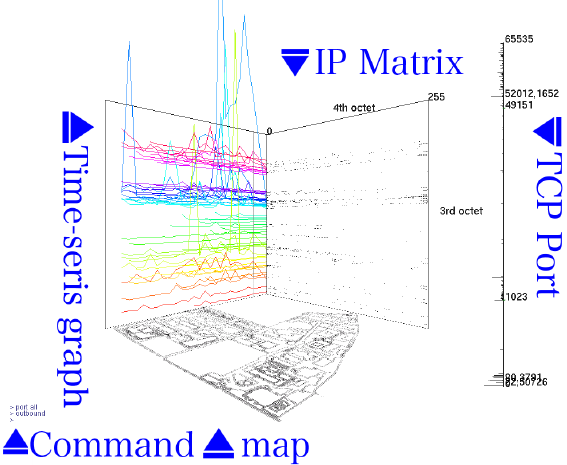
\includegraphics[scale=1]{integrated.png}
\vskip 0.5cm}}
\caption{\protect\label{integrated}Overview of integrated IDS visualisation system \cite{mukosaka2007integrated}. Newer events appear to the right of the time plane.}
\end{figure}

When in the configuration shown in Figure \ref{integrated}, the timeline plane shows events for the entire subnet x.y.x.*. Individual IP's can be chosen by shifting the timeline plane along the IP plane.
Filtering tools are made available to control what kinds of events are shown, though are not described in any kind of detail. port at least is usable to filter on. 

This system relies colour to distinguish ports on the timeline frame, which is easily subject to visual overload, as the human eye is not able to reliably distinguish fine differences in colours. Vertical position of the line indicates the number of events. With poorly described filtering systems and reliance on colour coding to distinguish ports, this system is extremely vulnerable to producing information overload. This leads to missing important events. the lack of data hiding creates visual clutter which can easily mask important intrusions composed of a small number of events. 

This system appears interesting as an attempt to correlate attack information with machine location through geoip systems. Where the number of events is "low enough" lines are drawn from IP plane to physical location on the lower plane. The exact number of lines drawn is not clear. 


\chapter{Progress}\label{C:progress}

\section{Design}\label{design}

Significant design work has been performed for this system at both the architectural level and user interface. Interface design is discussed in section \ref{screen_design}. 

I have chosen to implement a client server model for the system architecture, as this offers a strong separation into multiple loosely coupled modules. Given a client server architecture, and a desire for centralised data storage between multiple users a browser based approach was chosen. Using existing browsers leverages significant work done on secure network communications between client and server, as well as significant effort in sand-boxing (isolating from the rest of the computer) in-browser applications. This saves significant time and effort on implementing communication protocols and security. 

As there are relatively few programming languages available for use within the browser this significantly simplified the choice of languages and tool sets. See section \ref{langs}.

\begin{figure}[tbh]
\fbox{\parbox[b]{.99\linewidth}{
\vskip 0.5cm
\centering 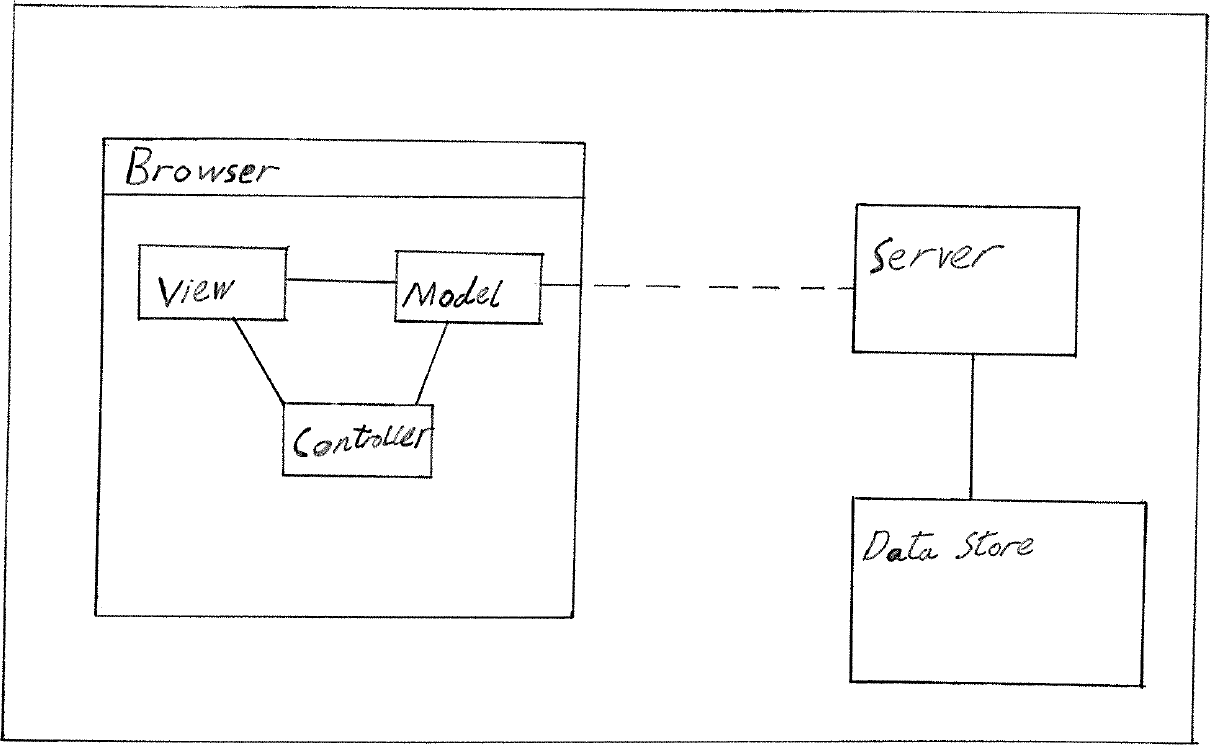
\includegraphics[scale=0.3]{blocks.png}
\vskip 0.5cm}}
\caption{\protect\label{spiral_plan}Block diagram showing proposed architecture of system. Note complete separation between server and browser. These may reside on separate machines.}
\end{figure}

Inside the browser there are three major components from an object oriented perspective. The view contains what is actually displayed on screen, this is implemented in HTML with SVG (Scalable Vector Graphics) for graphical components. The model stores the data and handles requests to the server as necessary. The controller is responsible for implementing user interaction with the system.

Communication between the client and server is handled through standardised protocols. The set of requests permissible is still to be defined. The server software is responsible for serving data to the client, performing data aggregation, and limited data mining. In order to provide data, the server communicates with the data-store. This communication is likely to take place through SQL to a database, though a modular design could permit creation of other storage interface modules.

Data aggregation is performed server side for two reasons. In larger networks, or over longer time periods, many megabytes of logs can be created, while text is highly compressible this still creates significant network overhead to transfer. Further, there are unanswered questions about how well the client will perform with potentially millions of events to manipulate. Slow data transfers or interaction due to processing time would be a significant usability hurdle. Performing data aggregation on the server bypasses both of these limitations. 

\subsection{User interface design}\label{screen_design} 
  
I have chosen to adopt a time based approach for the visualisation elements, as access attempt logs have a very strong time component. Some forms of unusual behaviour are evidenced only by unusual times for access attempts, or unusual durations of access for example. Most existing visualisations do not give much emphasis to the time relation between access attempts, preferring to focus on the links between source and destination addresses.

Two major approaches have been considered for displaying log entries.
Spiral view is an approach for displaying time series data mapped to a spiral, see figure \ref{spiral} where a straight line drawn from the outer edge to the center shows the same time at each level of the spiral \cite{bertini2007spiralview, chin2009visual}
These systems appear to be highly effective at displaying time series data in a fashion that supports easy detection of repeated patterns. 

\begin{figure}[tbh]
\fbox{\parbox[b]{.99\linewidth}{
\vskip 0.5cm
\centering 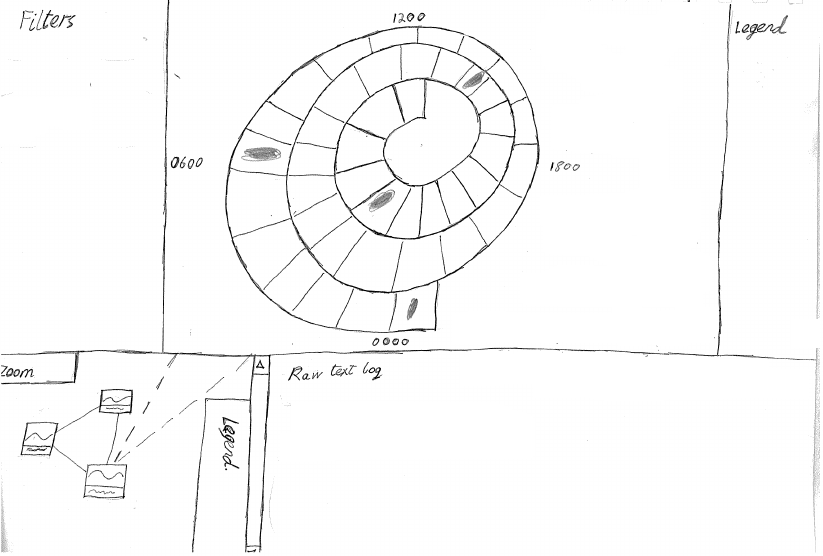
\includegraphics[scale=0.75]{spiral_plan.png}
\vskip 0.5cm}}
\caption{\protect\label{spiral_plan}Drawing showing proposed layout using spiralview for main focus. Black shading shows selection of an event with highlighting of related events.}
\end{figure}
 
However serious flaws in the results(\cite{chin2009visual}) of usability tests presented have lead to the rejection of this method. The error in question shows a table of results that directly contradict claims made in the text about how well spiralview supports the detection of patterns. The claims contradicted in the work are those directly bearing on the uses I had intended for the spiral layout. As this is a 300 hour project, I will not be attempting to repeat their work to clarify their findings. I attempted to contact the authors of the paper, and have as yet received no response.

This contradiction has lead to using a simpler and better understood layout for time series data. 

\begin{figure}[tbh]
\fbox{\parbox[b]{.99\linewidth}{
\vskip 0.5cm
\centering 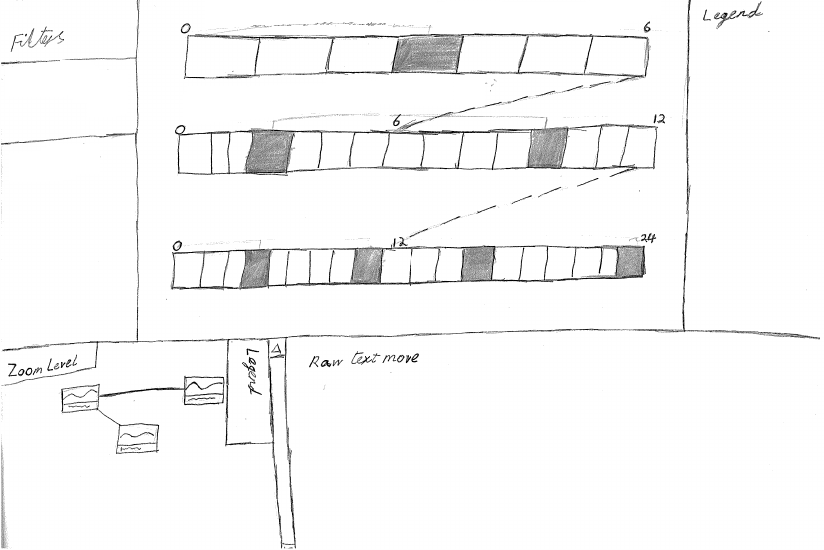
\includegraphics[scale=0.75]{lines.png}
\vskip 0.5cm}}
\caption{\protect\label{lines}Drawing showing proposed layout using multiple time lines for main focus. Black shading shows selection of an event, with highlighting related events.}
\end{figure}

Using block representation of data arranged linearly along a time axis.
Initial designs called for using a stacked representation where each layer represented twice the time of the previous layer.
This is proposed to show patterns as an element that repeats a growing number of times in each layer.
Tufte's work on small multiples \cite{tufte1983visual} suggests keeping each level of the stack to represent the same amount of time, with differing start and end points. Ie: if the range is 6 hours, the top bar starts at 0600, and runs to 1200, the one below it from 0000 to 0600..  and so on. This would show patterns repeating with a period less than the time range by showing in multiple bars. See Figure \ref{lines}.

I have been forced to consider data hiding techniques, as networks can become extremely busy, producing sufficient activity to overwhelm the user's ability to absorb information and detect meaningful patterns in the clutter. As I have chosen a time series based approach to displaying the data, I have chosen to use time binning to aggregate entities. This approach is extremely simple, with all entries in a short time period displayed as a single entity, with icons indicating some simple features of the hidden data. Such features include superuser accesses, abnormal numbers of failed access attempts, abnormally large numbers of access attempts, abnormal login locations for a user, abnormal login times for a user. Each time bin can be zoomed in on, allowing the user to see greater detail within the bin. For extremely busy systems and longer time periods there may be multiple levels of binning in play to aggregate sufficiently. This scheme reduces the visual complexity, while allowing easy access to detailed information about each incident. 

These last are the most complicated flags, as they require creating a profile of each user's access times over repeated access attempts. This complexity can produce false positives while the system is learning a new user's habits. and may be tripped up by a legitimate change in user habits.

\subsection{Tools and Languages}\label{langs}

I have chosen to use javascript with the d3 visualisation library \cite{bostock2011d3} for the client portion of the system. This was chosen as d3 is a very well supported visualisation library offering excellent support for dynamic data, animations, graph layouts and highly customisable charting. D3 also offers convenience methods significantly simplifying data requests from the server. While this does require learning a new language, a head start has been afforded through using these tools for another project. Assistance with learning through documentation and peers is excellent for javascript and d3 as many fellow students have used these tools extensively.  Javascript has excellent support across all major browsers and platforms, and is the defacto standard for interactive webpages. Drawbacks of Javascript -> dynamic typing, and implicit declaration allows for easy introduction of subtle and hard to debug errors. Major -> lack of locale support in js limits time display to local timezone only, or GMT. issues with datetime picker addon combined with lack of locale support forced fallback to local timezone only.

Java was another possible language for implementing the client. While this has the advantage of already knowing the language well, there were two significant drawbacks. Firstly, browser java plugins have a very long and poor security record, with many new vulnerabilities found each year. In an application where sensitive data is used, security is an important concern. Secondly, there is no library providing visualisation support comparable with d3, further to this, fewer students use java for visualisation projects, and graphics are significantly more difficult to write effectively in java.

Other libraries used -> 
JQuery -> extremely helpful for crossbrowser consistency, and simplification of DOM manipulation.
JQuery UI -> JQuery extension offering css based theming and UI widgets. somewhat helpful, though let down by some widgets (slider inability to be dragged by fill in vanilla JQueryUI). Theming hugely helpful, as JQuery developers make available a theme creator tool(themeroller) allowing even a relatively unskilled person to create a customised theme.
history.js -> unifies handling of HTML5 history api across browsers. some irritation as forces data reload on replaceState. this is insignificant due to amount of data transferred, and target usecase (on local network only).

Java 6 and Tomcat used for server side code, interfacing with MySQL database.
Used - jOOQ library for SQL query writing. this allows for cross database support, almost any RDBMS can be used with the existing server code, so long as the same schema is followed.

Tomcat -> webserver from apache foundation created as a server for java servlets. This provides access control, multithreading, resource access and handles the core networking processes for serving. One layer for a defence in depth. Easily configured to require SSL for all communications with client, and limit addresses able to connect at all.
Java servlets -> written in java 6 due to limitations of the tomcat version available at uni. Extremely easy to use and understand.

logfile parser written in java6, fairly simple and straightforward.

\subsubsection{Supporting tools}
Git -> distributed version control system. used to track code changes, and share codebase between uni and home.
GitHub -> site for sharing git repositories. Makes available an issue tracker which is integrated with git commit comments. Integration allows associating commits with issues, and closing issues from commits. this integration is extremely useful for debugging and tracking why changes were made.



\section{Evaluation}\label{eval}

Evaluation of the tool produced in this project will serve to determine if there is sufficient merit to the idea to justify further development work on the tool. If the evaluation determines that there is sufficient potential to justify the development work, future work can evaluate the effectiveness of the design in a more rigorous manner. I have chosen to perform an exploratory evaluation due to time limitations on this project \cite{Ellis:2006:EAU:1168149.1168152}. It's not possible to achieve a representative sample of sufficient size to have predictive power in the time available. This limitation strongly suggests against attempting to demonstrate conclusively the usefulness and usability of the system. 

Ethics approval has been sought for this experimental design. As of writing the application has been approved by the head of school and is before the committee.
\subsection{Evaluation Design}

Evaluation will be performed by means of a qualitative user study, with ideally 10 to 15 participants. 
Participants will be given a chance to familiarise themselves with the tool on a limited training dataset.
After familiarisation time, participants will be asked to answer four questions about each of two datasets.
For each of the 8 combinations a brief questionnaire will be completed, indicating opinions about the tool's performance in the task\cite{lewis1995ibm}. 
\subsubsection{Users}

As this tool targets domain experts in the security domain, I will be recruiting participants from the security industry, both on campus and off. I have pitched the experiment to students enrolled in NWEN405, which deals with computer security as a secondary source of participants. Students are less ideal, as their experience and domain knowledge are more limited than those that have been working in the industry for some time.

\subsubsection{Datasets}

Two datasets have been acquired for use in this experiment.
\begin{enumerate}
\item{Honeynet Forensic challenge 10 dataset \cite{forensic10}. This dataset is anonymised and public domain. The data presented here covers a single server, with low traffic (9MB covering mar 16 to may 2)}
\item{Anonymised logs from the Engineering and Computer Science network at Victoria University. This dataset is significantly larger, covering 3 servers and 2 weeks of time on a high traffic network. Exact data size is not yet known, as the data collection process is ongoing at time of writing.}
\end{enumerate}

\chapter{Evaluation}\label{eval}

Evaluation of the tool produced in this project served to determine if there is sufficient merit to the idea to justify further development work on the tool. If the evaluation determines that there is sufficient potential to justify the development work, future work can evaluate the effectiveness of the design in a more rigorous manner. I have chosen to perform an exploratory evaluation due to time limitations on this project \cite{Ellis:2006:EAU:1168149.1168152}. It is not possible to achieve a representative sample of sufficient size to have predictive power in the time available. Two factors limit the ability to achieve a representative sample in the time available, taking part in the experiment requires between 1 and 1.5 hours. a further 1 to 1.5 hours is required to grade and analyse the data. Further, there is a relatively limited pool of potential participants as the tool is targeted at security experts. This limitation strongly suggests against attempting to demonstrate conclusively the usefulness and usability of the system. Small, exploratory evaluations have advantages in cost and time required. With small numbers of participants, the evaluation can be carried out in a short time. These exploratory evaluations can also be useful to discard non-viable approaches before significant development effort has been spent. Care should be taken to avoid evaluating too early however, as the unfinished nature of the product can distort results. 

Ethics approval has been granted for this experimental design.<ref appendix> 

\section{Evaluation Design}

Evaluation was performed by means of a qualitative user study, with 6 expert participants. Two datasets were used, representing different sizes and complexities of system. Each participant was presented with 4 tasks to complete for each dataset. Time taken and accuracy was recorded for each task, along with a 3 question usability survey. 

\subsection{Users}

As this tool targets domain experts in the security domain, I have recruited participants from the security industry, both on campus and off. I have pitched the experiment to students enrolled in NWEN405, which deals with computer security as a secondary source of participants.
--Expand this section, leave full personae in appendix.
4 participants from industry, 3 at VUW
All four professional participants had security issues as at least a portion of their day jobs, and could be expected to be involved in log analysis tasks on a regular basis.
2 students.  Both students had strong security and networking backgrounds.

\subsection{Datasets}\label{data}

Two datasets have been acquired for use in this experiment. Both datasets represent real systems exposed to the public internet. 
\begin{enumerate}
\item{Honeynet Forensic challenge 10 dataset \cite{forensic10}. This dataset is anonymised and public domain. The data presented here covers a single server, with 35K log entries covering March 16 to May 2}
\item{Anonymised logs from the Engineering and Computer Science network at Victoria University. This dataset covers three servers, for two disjoint weeks and 74K log entries.}
\end{enumerate}

While both datasets were anonymized, anonymization procedures were different. The honeynet dataset is publically available in an anonymized form \cite{forensic10} whereas the ECS dataset was recorded from internet facing servers in the ECS network. The latter dataset required anonymization of both usernames and IP addresses. IP addresses were anonymized with cryptoPAN <ref> a prefix preserving IP address anonymization tool extended with support for IPv6 addresses. Usernames were anonymized through a very simple scheme, where each username was replaced with the string "user" + a unique number. ie: user4 is a different person to user5.

The ECS dataset was altered, to introduce a successful scattergun attack on one server. ThIs was introduced, as there were no naturally occuring successful attacks.  The introduced scattergun attack had a very small attack signature, with only 204 log entries involved, of 4.7K entries for that day.
<check actual results, some successful root attacks on honeynet had similar sized signatures, some much larger, though with more noise for larger datasets.>
this needs more analysis.

\subsection{Setup}
Participants were provided with one of two machines
\begin{itemize}
\item{Dell Optiplex 9010 with an i7-3770 CPU and 8Gb of ram running Arch linux 3.7.5}
\item{Dell Optiplex GX760 with a Core2 Duo CPU and 4GB ram, running Arch linux 3.7.5}
\end{itemize}
Both systems had chrome 26.0.1410.63 as the browser.

Different hardware was used, as I was not able to secure the same room for all participants. 
While there are significant differences in the hardware capabilities, I do not believe that these are significant
as the design of the tool does all memory and computationally intensive work server side, with only a few kilobytes of data transferred for each view. This results in a relatively small memory footprint, and limited resource requirements for the client computer.
More significant is the consistent OS and browser versions, as javascript behaviour can be influenced strongly by browser implementation. Though this is relatively rare for javascript behaviour to change significantly between major browser versions, this is not unknown. By ensuring both systems used the same OS and browser, this possible source of error is eliminated.

The experiment was conducted in a quiet lab, with only the experimenter and subject present. Each question was allocated an 8 minute maximum, based on test runs with a supervisor. Audio recordings were made as a record of events during the experiment as an addition to handwritten notes. 

\subsection{Procedure}
Participants were given up to ten minutes to familiarise themselves with the tool, and how it behaves. After familiarisation, participants were asked to answer four questions about each of two datasets. For each of the 8 combinations a brief questionnaire was completed indicating opinions about the tool's performance in the task\cite{lewis1995ibm}.
Questions were presented to users in randomised order. This was done in order to avoid learning effects distorting results for the first question.

\begin{enumerate}
\item{Find an instance of a successful brute force attack on root.}
\item{Find an instance of a successful scattergun attack.
(an instance where the attacker attempts many common username/password pairs at random).}
\item{Find an instance of a legitimate user logging in from an abnormal location.}
\item{Find an instance of a legitimate user logging in at an abnormal time.}
\end{enumerate}

Questions 1 \& 2 are based on the most commonly found attack signatures in SSH logs. with many botnets and automated systems carrying out brute force or scattergun attacks against any IP address responding to connection requests. As these attacks are very common and can lead to serious compromises, as shown in the Honeynet dataset, determining success or failure of such attacks is a core function of any log analysis tool. 

Questions 3 \& 4 are based in finding anomalous behaviour by legitimate users. Anomalous behaviour by legitimate users can be an indication that their account has been compromised, or that they are attempting to carry out actions that would not be permitted in usual usage. <Badly worded. I mean they might be trying to compromise the system or data stored there.>. 

Tasks 1 through 4 were based on questions 1 \& 2, with tasks 1 \& 4 using the ECS dataset, and tasks 2 \&3 using the Honeynet dataset.
Tasks 5 through 8 were based on questions 3 \& 4, with tasks 5 \& 7 using the ECS dataset, and tasks 6 \& 8 using  the Honeynet dataset. 

Timing and accuracy for each task was recorded. 
Time was measured manually, by means of a stopwatch. While stopwatches are hard to use for subsecond accuracy, this is not required for a study of this type. Errors in timing on the order of 5 seconds are acceptable.

For each task a date, time, source IP and where applicable username involved were recorded. This combined with the dataset provides sufficient information to allow checking of answers for accuracy from the raw logs, database directly, or using the tool. 

\subsection{Threats to validity}
 Students are less ideal, as their experience and domain knowledge are more limited than those that have been working in the industry for some time.
Dataset size - both in 10K order of magnitude, this limits our ability to speculate about how the tool will scale to 100K+ sizes. 
Small number of participants - unable to control effectively for demographic variations, or ensure 

\section{Results}

Each Task was graded for accuracy, and time taken to complete the task was measured.
\begin{table}[tbh]
\centering
\begin{tabular}{l|*{12}{l|}}
Task & 
\multicolumn{2}{|c|}{Participant 1} & 
\multicolumn{2}{|c|}{Participant 2} & 
\multicolumn{2}{|c|}{Participant 3} & 
\multicolumn{2}{|c|}{Participant 4} & 
\multicolumn{2}{|c|}{Participant 5} & 
\multicolumn{2}{|c|}{Participant 6} \\
\hline
Task 1 & 3:05 & \cmark & 5:46 & \xmark & Invalid & \xmark & - & \xmark & - & \xmark & - & \xmark \\
Task 2 & - & \xmark & - & \xmark & 2:26 & \cmark & 2:09 & \cmark & 3:55 & \cmark & 3:08 & \cmark \\
Task 3 & 5:10 & \cmark & - & \xmark & 4:18 & \cmark & 4:51 & \cmark & 8:00 & \cmark & 2:20 & \xmark \\
Task 4 & - & \xmark & - & \xmark & 4:18 & \cmark & 3:18 & \xmark & - & \xmark & - & \xmark\\
Task 5 & 1:09 & \cmark & 1:22 & \cmark & 1:07 & \cmark & 0:39 & \cmark & 1:04 & \cmark & 1:10 & \cmark \\
Task 6 & 0:31 & \cmark & 1:07 & \cmark & 1:02 & \cmark & 1:13 & \xmark & 1:00 & \cmark & 2:15 & \cmark \\
Task 7 & 0:45 & \cmark & 1:59 & \cmark & 0:42 & \xmark & 0:44 & \cmark & 2:06 & \cmark & - & \xmark \\
Task 8 & 0:32 & \cmark & 1:10 & \xmark & 1:32 & \xmark & 1:07 & \cmark & 1:15 & \cmark & 0:55 & \cmark \\
\end{tabular}
\caption{Time taken to complete each tasks}
\label{res_times}
\end{table}

Observation of participants working on tasks 1 through 4, and participant comments suggest that difficulty in navigating the timeline was a significant issue for carrying out these tasks.
Task 1 involved finding a brute force attack which compromised root on the ECS dataset. There was no such attack present in the dataset. It's well known that demonstrating the absence of something can be significantly harder than the presence.<justify this>. I believe the combination of navigational difficulties with increased task difficulty is the cause of the very high failure rate for this task, with only one participant successful.

Task 4 involved participants looking for a successful scattergun attack in the ECS dataset. why was this so hard? Poor navigation support caused problems, relatively small attack signature easily swamped in other data.

Tasks 2 \& 3 were to find a brute force and scattergun attack respectively on the Honeynet dataset.
There were multiple successful brute force attacks on the Honeynet dataset, and scattergun attacks with much larger attack signatures (higher number of attempts). These questions were quickly and reliably answered by all but one participant. Poor accuracy, and significantly slower times with ECS data coupled with observations of participants attempting these tasks suggest that navigation difficulties and limited filtering options were a greater issue in the more complicated dataset, with smaller attack signatures, and greater noise. 

Participant 2 had a great deal of difficulty in identifying brute force and scattergun attacks on both datasets. Feedback and observation of the participant in action suggest severe difficulties with navigation, combined with the lack of ability to hide all attempts from a specified set of IP addresses caused significant difficulties for this participant.

Participant 2 commented that in the normal course of investigating such incidents using tools such as grep, he would build up a blacklist of IP's to hide from results as they were fully investigated and discarded.
The tool as currently implemented does not support this. Participant 2 has significantly more experience in analysing sshd logs using traditional tools where stronger filtering tools are available, such as regular expressions. 

\section{Discussion} 
\begin{enumerate}
\item{Improved navigation through timeline. Users complain that it is easy to get lost when zooming. Animations may ease this transition. (possibly animate zooming in by expanding target bin to fill timeline, then chunking into new bins?)}
\item{Improved filtering of results by IP. several extra features are requested here, with the ability to filter by subnet, as well as hiding IP's (inverse of IP of Interest filter.)}
\item{Ability to filter connections by authtype, ie : excluding hostbased when looking for a successful brute force attack.}
\item{Improve performance of abnormal time and location detection, reduce false positives and spurious results by suppressing alerting on invalid or failed attempts. This will significantly cut down the number of abnormalities reported, reducing the false positive rate significantly.}
\end{enumerate}

include comparison with goals here.. how well did we meet them?
\begin{enumerate}
\item{Effective use of information hiding to prevent information overload.}
\item{Prevent masking of important data in noise or hiding. failed, more work required on filtering and clustering}
\item{Provide strong filtering and highlighting options. weaker than ideal, more work needed, performance dependent on exploration style and ability to maintain mental map of data.}
\item{Show surrounding context for anomalous accesses.}
\item{GeoIP support to add context to login attempts. geoIP results used in clustering algorithm, but not directly displayed.}
\item{Allow the user control over which machine is monitored at any given time. -included as dropdown selector, may have some scale issues for networks with many machines to monitor. no ability to select multiple machines currently, though dropdown easily expanded to allow this.}
\item{Show network context for currently monitored machine. dropped for lack of time}
\item{Performance capable of handling millions of events without perceptible delays. - untested, but unlikely due in part to network latency and javascript performance issues. did not have sufficiently large dataset to test performance with more than $10^3$ magnitude.}
\item{Extensible log parsing: don't prevent extension to other similar log types.}
\end{enumerate}

\section{Future work}
what do we need to do from here?
address known bugs.
address discovered weaknesses
 - add more filter types
 - add mechanism for excluding addresses from results.
 - refine clustering algorithm to reduce false positives. 
 - animate transitions to assist navigation.
maybe some work on performance?
critical - once bugs and new features addressed, perform a more complete evaluation
higher n, with actual statistical power, and much more variety of datasets. allow more training time, and some learning questions.
\chapter{Plans}\label{C:future}

\section{Design}
As I'm building the tool as a web based system, I have been forced to use a client server model.
Use of web based systems leads to some security concerns regarding access control and system robustness.

Using web based technologies has the advantage of tapping into significant existing work in visualisation libraries 
and remote database access, see Section \ref{tools} for details.

Significant work remains to be done on the database schema for storing SSHD log entries, These entries are highly structured, which allows for a relatively simple parser to break down into usable form. As existing designs call for a raw text view to accompany the main visual components (see Section \ref{screen_design}) I propose to store the raw log entry as a text field  within the database. Some design work is required to describe a storage mechanism for information about individual users and network structure. The minimum information required would be typical access times and locations for users and server names, locations and uses for machines. I do not forsee significant difficulties in designing a storage layout for this data.

Design of server side code and functions remains to be carried out, though I plan to perform the majority of data processing server side, due to concerns about javascript and browser performance when hundreds of thousands to millions of elements are being manipulated. 

\section{Security Concerns}
As I'm building the tool as a client server model, accessed through the browser
there are several security concerns to be considered in a deployment of the system.
The database will contain a significant amount of privileged information about network security
such as machine names and addresses, valid account names, and authentication methods used in the system.

This data would be extremely useful to malicious users or outside intruders. 
This leads to a need to ensure that access to this database is controlled through a robust authentication system.
Ideally the web server hosting the tool should not be accessible to the outside world at all. Within the organisation's private network access should be restricted tightly to only those users with a definite need to have access. 
Secured connections must be used for all communication between client and server to limit the opportunity for malicious individuals to snoop on the data in transit.

Security of the serverside code will be considered from the beginning of the design and implementation process
as this code must be able to resist any malicious access attempts. Through input sanitation and bounds checking should serve to close the majority of possible vulnerabilities.

Client side code contains no data, and so is significantly less critical to secure, as the database systems should deny access without valid credentials. Ideally host based authentication could be used. However, implementing a robust access control scheme does not fit within the scope of this project, and will be left for future development.

\section{Implementation}

Implementation of the tool remains to be started, this along with evaluation comprise the majority of remaining work to be performed.
I will be using a github repository for version control and backup purposes.

\subsection{Tools and Languages}\label{tools}

As I have elected to use a client server model with the client residing in a web browser a suitable server side language must be chosen to allow database connectivity. I am largely unaware of the strengths and weaknesses of various server side languages. Further research is needed to decide between the various possibilities. Java appears on the surface to be a strong contender due to language familiarity and strong tool support through eclipse. Tomcat provides a solid framework for interfacing web requests with java code.
Many other languages remain, such as perl, php, and ruby or even serverside javascript. Each of these languages requires learning a new language effectively from scratch, this is a significant time cost on a short project. 

\subsection{Testing}
Automated testing of user interfaces remains problematic, with many tools suffering from severe fragility where UI layout is modified. In most testing libraries, mous interaction is recorded at test design, then played back artificially on execution, This causes severe fragility as if a control or button moves the recorded mouse movements will miss the button, causing test failures. Further research is needed to find a testing library suitable for testing, however the test automation tool created by Dojo appears useful \cite{dojo2013test}.

\section{Timeline}

I will be taking a couple of days as a complete break from university work following my exams on the 15th and 17th of June, with work on the project resuming on 19th June. Figure \ref{gantt} shows a Gantt chart breaking down my plans for the remainder of the work to be completed.  I expect to be done implementing the tool early in second trimester, with at least a month left after evaluation is complete to write up my final report before end of teaching trimester 2.
  
\begin{figure}[tbh]
\fbox{\parbox[b]{.99\linewidth}{
\vskip 0.5cm
\centering 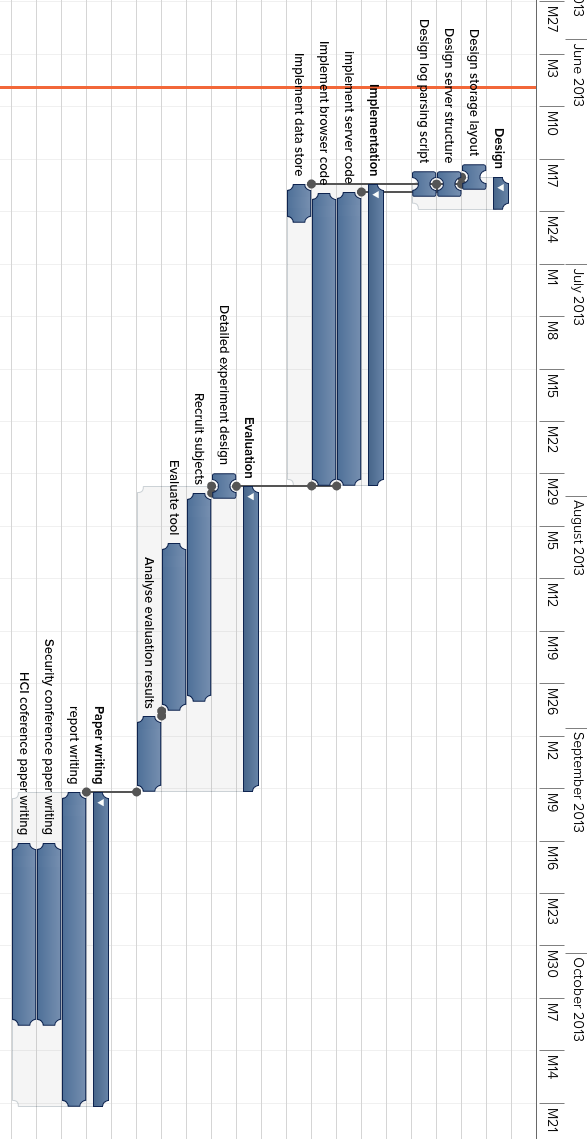
\includegraphics[scale=0.75]{gantt.png}
\vskip 0.5cm}}
\caption{\protect\label{gantt}Gantt chart showing breakdown of future work into major sections. The design group is all sub day tasks.}
\end{figure}

\subsection{Risks}

Several notable risks remain to this project.
\begin{description}
\item[Languages:] Learning a new programming language always carries risks of unexpected setbacks or difficulties in completing tasks due to lack of familiarity with language features and libraries. This can be mitigated through choosing languages appropriate to the tasks, ideally already well known languages. 
\item[Experiment Participants:] User evaluations always carry an element of risk in recruiting a suitable number of participants in the time available to complete the study. This can be mitigated through an early start to the recruitment process, and well chosen incentives. 
\item[Ethics approval:] User experiments carry an element of risk, as if ethics approval is delayed significantly, this will cause severe dislocation to the planned timeline, which may limit the evaluation after approval is gained. This is unlikely as approval has been sought already, and the application is before the committee.  
\end{description}


%%%%%%%%%%%%%%%%%%%%%%%%%%%%%%%%%%%%%%%%%%%%%%%%%%%%%%%

\backmatter

%%%%%%%%%%%%%%%%%%%%%%%%%%%%%%%%%%%%%%%%%%%%%%%%%%%%%%%


%\bibliographystyle{ieeetr}
\bibliographystyle{acm}
%\bibliography{/u/students/leliel/Courses/ENGR489/reports/project}
\bibliography{C:/Users/Lelitu/Uni/ENGR489/reports/project}

\end{document}
